\section{Procedure for the safety assessment}
\label{sec:procedure}

\begin{figure*}
	\centering
	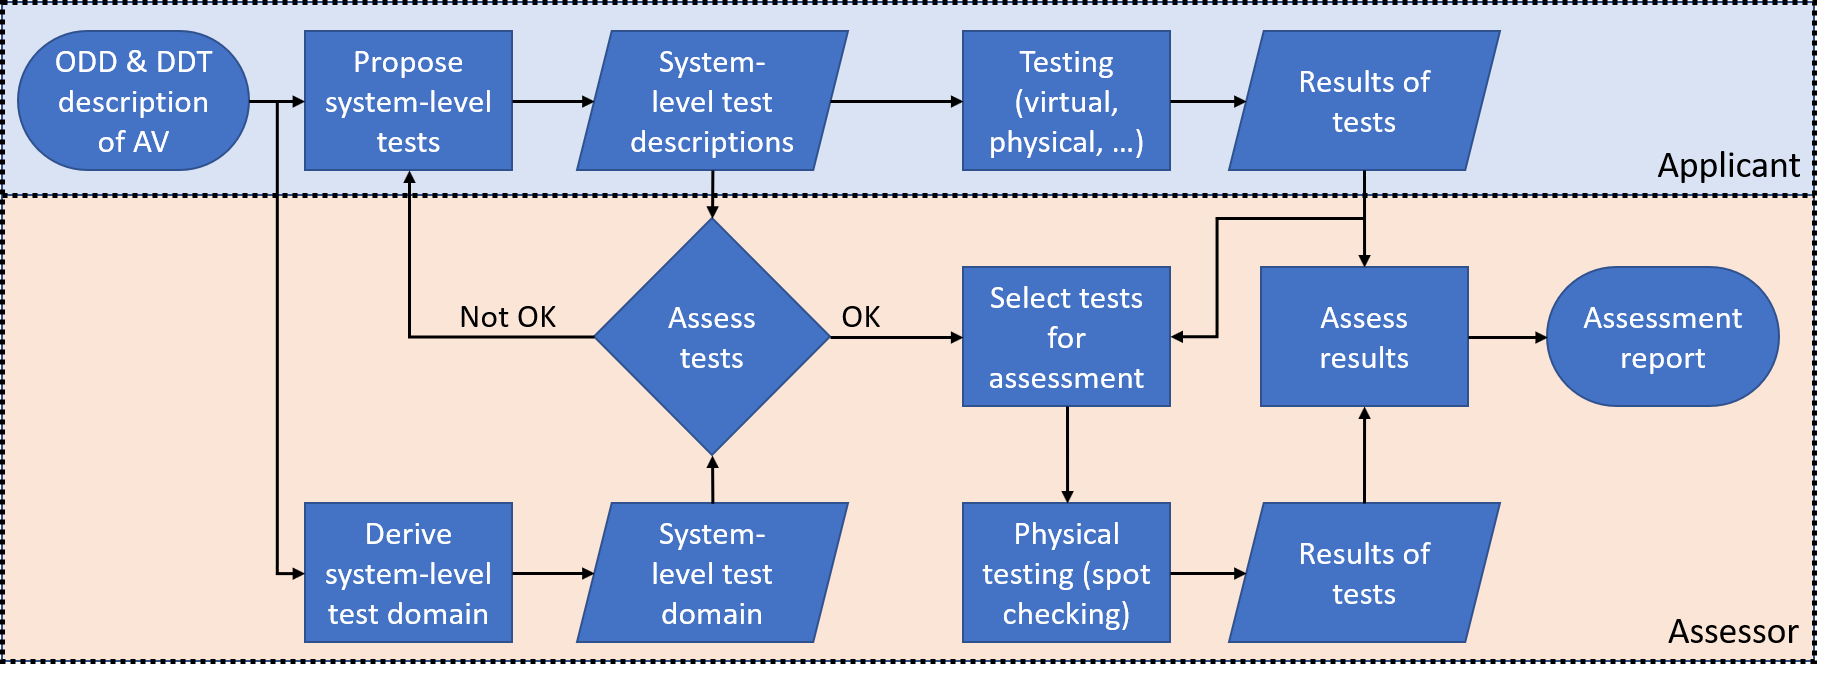
\includegraphics[width=\linewidth]{figures/procedure2}
	\caption{Proposed framework for the safety assessment of an autonomous vehicle (AV).}
	\label{fig:procedure}
\end{figure*}

This paper assumes that many of the relevant tests for the safety assessment are performed in a virtual simulation environment that is controlled by the applicant. The proposed procedure intends to consider all results, both from virtual simulation and from actually performed physical tests. Where the assessor does not have access to the required models of the AV under test, the assessor will have the capability to perform physical tests on the AV. How to balance between the different results in the assessment, considering virtual and physical test results of the applicant and physical test results of the assessor is schematically presented in \cref{fig:procedure}. Each rectangular block represents an action. The procedure distinguishes between actions for which the applicant is responsible and actions for which the assessor is responsible. The procedure consists of the following actions:
\begin{enumerate}
	\item The first action is to derive which system-level tests need to be performed with reference to the ODD and DDT of the AV under test. Here, “system-level” is mentioned explicitly, because it is assumed that also in case of a failure of any of the subsystems, the AV would fail the system-level tests. Note, however, that it is advised that the applicant ensures that each of the subsystems underwent a rigorous assessment before applying for the AV assessment. 
	\item If the derived tests are acceptable, the next action is to select the tests for the assessment. Here, a distinction is made between tests for which the applicant is fully responsible and physical tests that are conducted by the assessor. The latter will focus more on spot checking.
	\item Once the tests are selected, these tests need to be conducted. The results of these tests will be described using prescribed metrics. Note, however, that these metrics may not contain too much information as it is assumed that the applicant does not want to disclose details of sensor and system implementation or even detailed test results because of the proprietary or confidential information contained in these results. 
	\item The final step is to assess the results from the tests and to formulate an advice for the authority on whether the AV is ready for deployment and under which conditions.
\end{enumerate}

In the following sections, each of the actions are further detailed. We end this section with a short note on monitored deployment in case of a successful completion of the assessment.



\subsection{Deriving test descriptions}
\label{sec:test descriptions}

Based on the ODD and the DDT of the AV, the tests are derived. Following the same reasoning as \textcite{stellet2015taxonomy}, a test is an evaluation of:
\begin{itemize}
	\item a statement on the system-under-test (test criteria; what are we going to evaluate using the test);
	\item under a set of specified conditions (test case; how are we going to evaluate the test criteria);
	\item using quantitative measures (metrics; how to express the outcome of the test quantitatively);
	\item and a reference of what would be the acceptable outcome (reference; when is the outcome acceptable).
\end{itemize}

Since the applicant has designed and developed the AV, it is expected that the applicant has a clear notion of the tests that are required for a complete assessment of the AV and which the AV should appropriately handle. Similarly, if the set of relevant test descriptions is not complete during the development of the AV, it is conceivable that the AV will not operate safely for all circumstances possible within the ODD. 

Although it is expected that the applicant provides all relevant test descriptions, it is important that the applicant and the assessor discuss these test descriptions, and that a check is made whether or not the test descriptions are complete and cover the ODD sufficiently. If an important test description is missing, it is conceivable that the AV is not specifically designed to pass the corresponding test. In order to assess the completeness of the test descriptions provided by the applicant, the assessor needs to define the test domain for the relevant system-level test descriptions and use these to investigate if any important test descriptions are missing. Here, the so-called test domain refers to a more high-level description of the range of tests that are expected, rather than an enumeration of the large number of relevant tests.

If it turns out that the test descriptions that are provided by the applicant are not complete, the process needs to be restarted, as indicated by the ``Not OK'' line in \cref{fig:procedure}. On the other hand, if the test descriptions are deemed to be complete enough, the assessment proceeds to the next step: selecting tests for the assessment.



\subsection{Selecting tests for the assessment}
\label{sec:selection}

In principle, the applicant is expected to provide results for all tests. In the next section, we explain how these results may look like. Based on these results, tests are selected for the physical testing performed by the assessor. This is indicated by the arrow pointing from ``results of tests'' of the applicant to ``select tests for assessment'' in \cref{fig:procedure}.  

A test is selected for physical testing by the assessor if any of the following three statements are true:
\begin{itemize}
	\item The applicant does not provide a result. Although the applicant is expected to provide results for most tests, it might be possible that there are some tests for which the applicant does not have the resources to perform the tests reliably, for example if specific tooling is required. Note, however, that if the applicant does not provide results for too many tests, the assessment automatically results in a fail.
	\item The result seems inconsistent. If there is sufficient reason for the assessor to not confide in the result provided by the applicant, the test can be performed by the assessor to check the result provided by the applicant.
	\item The test is selected for spot checking. The main reason to perform spot checking is to assess the fidelity of the results provided by the assessor.
\end{itemize}
The process of test selection is summarized in \cref{fig:selection}.

\begin{figure}
	\centering
	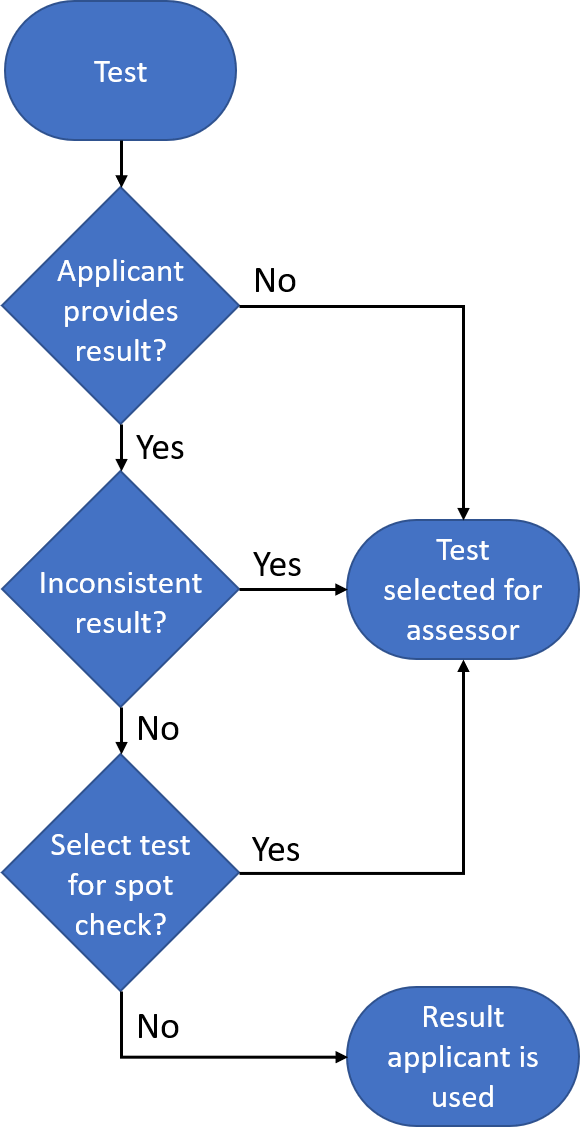
\includegraphics[width=.65\linewidth]{figures/test_selection}
	\caption{Decision scheme for the selection of a test for physical assessment by the assessor.}
	\label{fig:selection}
\end{figure}



\subsection{Testing}
\label{sec:testing}

As explained in the previous section, the applicant is expected to provide results for most tests. However, it is assumed that the applicant does not want to disclose detailed test results. Therefore, a rating scheme is proposed. Using a specific metric for each test, three references are defined: an acceptable result, a fair result, and a good result. If the result of the test is worse that the acceptable result, a ``fail'' is reported. If the result passes the acceptable reference but not the what is defined as a fair result, an ``acceptable'' is reported. Similarly, a ``fair'' is reported if the result is between a fair and a good result. If the result is better than what has been defined as a good result, a ``good'' is reported. This is schematically shown in \cref{fig:rating}. 

\begin{figure}
	\centering
	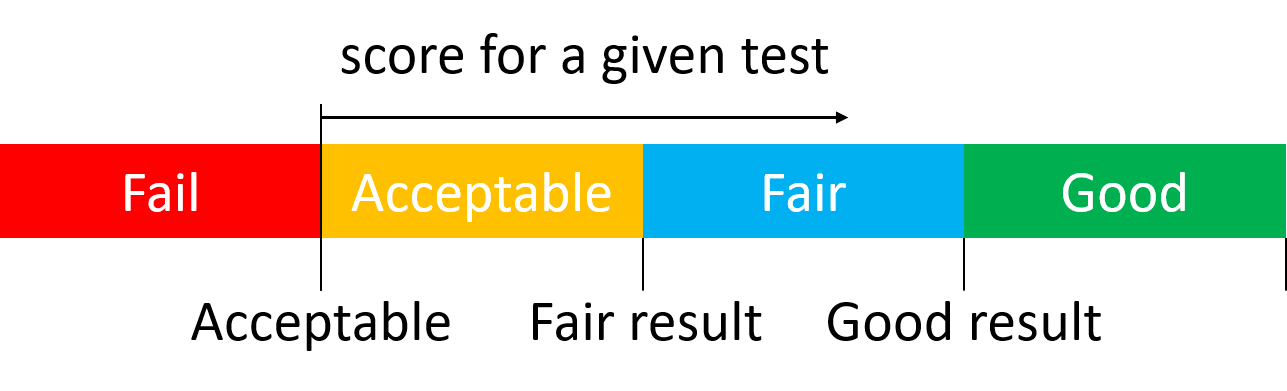
\includegraphics[width=\linewidth]{figures/rating}
	\caption{Different scoring options per test.}
	\label{fig:rating}
\end{figure}

In principle, the applicant is free to choose any method to derive the results. However, considering the large number of tests, the use of virtual simulations seems inevitable. In practice, it is expected that a both virtual simulations, physical tests, and a combination, such as hardware-in-the-loop testing, is used to determine the test results.

On the other hand, the tests by the assessor are performed physically. The main reason for this is that virtual simulations are ruled out as that would require the applicant to provide a model of the AV, which is expected to be impossible because of proprietary reasons.



\subsection{Assess results}
\label{sec:assess results}

The following assessment results are distinguished per test:
\begin{itemize}
	\item In case the test results show that for the specific test the AV performs acceptable (i.e., ``acceptable'', ``fair'', or ``good'', see \cref{fig:rating}), the test is passed. If this is not the case, then the specific test fails.
	\item Inspired by IATF~16949 on automotive quality management \autocite{IATF16949}, a passed test may result in a non-conformity. An “acceptable” result automatically leads to a non-conformity (NC). This means that the response of the AV deviates substantially from  response that is qualified as “good”, but the deviation is not severe. Since the AV meets the minimum requirement for this test and consequently safety is not compromised, there is no reason to fail the AV based on this test. Nevertheless, an NC is issued to indicate that the applicant is asked to consider improvements, e.g., for a next version of the system.
	\item In case the test is also performed by the assessor and the corresponding result is worse than the reported result of the applicant, this also leads to a NC.
	\item The assessment of a test result might come with an observation (OB) that needs consideration of the applicant. 
\end{itemize}

If a test results in a fail, then either the assessment results in a negative advice of the assessor to the authority or it is advised to only allow for deployment of the AV under certain conditions. For example, if the only tests that are failed consider low-light conditions, the AV might be deployed under the condition that it operates only from sunrise till sunset. 

NCs and OBs do not lead to an immediate fail of the assessment. However, it is likely that they lead to a fail in a future assessment, e.g., when test criteria become increasingly demanding, and the applicant does not appropriately consider such NCs or OBs. NCs provide information to the applicant on how requirements might develop in the future, which, consequently, gives direction and motivation on continuous improvement of AVs regarding safety. On the other hand, many NCs – the AV barely passes the test in many cases – might mean that safety is compromised and, therefore, it might also result in a negative advice of the assessor to the authority regarding the deployment of the AV.

Note that when many NCs are observed, the AV probably will not be able to pass all tests if all tests would be performed physically by the assessor. Theoretically, this is however still possible. To minimize the risk of having an AV that passes all tests, but with many NCs, a system using demerit points is introduced. The AV starts with, e.g., 100 points, and in the assessment, 1, 2, or 3 points are subtracted for each NC, depending on the severity of the NC. Once the number of points for the AV are reduced to 0, then the AV is indicated to have failed he assessment because of an overrun of NCs. The numbers given here are merely provided as an example.



\subsection{Monitored deployment}
\label{sec:monitored deployment}

A successful completion of the proposed assessment might result in the approval for the deployment of the AV under the condition that the behavior of the AV on the road is continuously monitored. We propose that during such a deployment phase, the applicant is required to upload detailed driving data to allow for monitoring the AV behavior. This is implemented for two reasons:
\begin{itemize}
	\item After completion of the assessment pipeline, road and/or vehicle authorities may require the monitoring of safety continuously when driving on the public road.
	\item The uploaded data may be used to improve the generation of tests and the selection of relevant test cases for a particular AV, as is possible that some tests have been overlooked during the initial assessment process or that situations on the road gradually change with changes in traffic, e.g.because of the introduction of new mobility systems.
\end{itemize}

The feedback to the data acquisition element allows for ongoing learning and improvement of the standards and assessment systems, while being able to adapt to new types of transportation such as personal mobility devices. For example, additional test cases could be identified and incorporated into future safety assessment procedures. A deployment might consider new operational areas, the extension of the scenario database with scenarios that potentially differ between such areas would then be covered. Moreover, to obtain a scenario database that is `complete', i.e., statistically accurate, it is expected that operational data collection is required over an extended period, which most probably will not be realized before the deployment is operationalized. In other words, the imperfection of the assessment framework should not become a barrier for the introduction of new safe mobility solutions onto the market, in case these devices are tested to be safe for all currently known conditions. The assessment method, especially the step regarding monitored deployment, supports the continuous increase in knowledge on the state-of-the-art of road safety and herewith prepares the safety assessment method to be sustainable for the future.
